\documentclass[12pt,oneside]{report}
\usepackage[UTF8]{ctex}
\usepackage{float}

%%%%%%%%%%%%%%%%%%%%%%%%%%%%%%%%%%%%%%%%%%%%%%%%%%%%%%%%%%%%%%%%%%%%%%%%%%%%%

% Definitions for the title page
% Edit these to provide the correct information
% e.g. \newcommand{\reportauthor}{Timothy Kimber}

\newcommand{\reporttitle}{Automated Research Poster Layout Tool}
\newcommand{\reportauthor}{Zihan Yu}
\newcommand{\supervisor}{Thomas Lancaster}
\newcommand{\degreetype}{Advanced Computing}

%%%%%%%%%%%%%%%%%%%%%%%%%%%%%%%%%%%%%%%%%%%%%%%%%%%%%%%%%%%%%%%%%%%%%%%%%%%%%

% load some definitions and default packages
\input{includes}
\usepackage{booktabs}
\usepackage{tabularx}
\usepackage{array}
\usepackage{ragged2e}

\newcolumntype{Y}{>{\RaggedRight\arraybackslash}X}

% load some macros
\input{notation}

\date{September 2026}

\begin{document}

\input{titlepage}

\pagenumbering{roman}
\clearpage{\pagestyle{empty}\cleardoublepage}
\setcounter{page}{1}
\pagestyle{fancy}


\chapter*{Abstract}
\addcontentsline{toc}{chapter}{Abstract}

Academic posters must compress research content, integrate figures and tables, and organize information within a limited single-page space. Their automatic generation therefore requires not only text summarization, but also document parsing, content selection, image–text matching, and layout planning. This project presents a modular system that converts research paper PDFs into editable PPTX posters. The system parses each paper into a structured representation, selects relevant sections, generates poster-oriented summaries while preserving key facts, and matches visual materials to textual content using captions, context, and explicit references. A content-aware recursive binary-tree layout allocates space according to textual and visual requirements, while local fitting reduces overflow and excessive whitespace. The structured intermediate states also make content and layout decisions easier to inspect and adjust.

\vspace{1em}

The system was evaluated on 40 papers from the Paper2Poster dataset, producing 120 poster artifacts. It was compared with a fixed-template baseline and a one-step Direct LLM baseline across content coverage, factual fidelity, and visual quality. The proposed method preserved more paper-specific details than Direct LLM on PaperQuiz detail questions and handled complex content structures more effectively than the fixed-template approach, especially in reducing overflow and inefficient space usage. Direct LLM achieved higher overall Faithfulness and Visual Scores, while the fixed-template method remained stable on structurally regular papers. These results show that automatic poster generation involves clear trade-offs between information density, factual reliability, and visual presentation. Overall, the project demonstrates the value of treating paper-to-poster generation as a structured and controllable process, producing an editable poster draft that automates much of the initial content organization and layout while preserving flexibility for final author refinement.

\chapter*{Acknowledgements}
\addcontentsline{toc}{chapter}{Acknowledgements}

First and foremost, I would like to express my sincere gratitude to my supervisor, Thomas Lancaster, for his guidance and feedback throughout this project. From determining the research direction to the final implementation, whenever I found myself uncertain about how to move forward, he always gave me encouragement and recognition for the work I had done, while offering practical and constructive advice. His support gave me greater confidence and determination as the project progressed.

\vspace{1em}

I would also like to thank Imperial College London and the Department of Computing for providing me with invaluable learning resources and facilities throughout this year of study.

\vspace{1em}

Thank you to the UK, and thank you to London. I can still vividly remember how I felt when I arrived in London alone a year ago. I was surrounded by an unfamiliar language and an unfamiliar environment, and everything made me feel nervous. Yet I still remember the smiles I received whenever my eyes met those of strangers passing by. I am grateful to every stranger who offered me kindness and help during this year.

\vspace{1em}

I would like to thank my family. It is because of your wholehearted support that I have had the opportunity to see a bigger world. You have always been the strongest support behind me, giving me the courage to keep moving forward. I feel incredibly fortunate to have you.

\vspace{1em}

I would also like to thank Shangjie and Sihan. Every time we are together, I feel a sense of comfort and familiarity. We have experienced so much together and shared both the joys and the difficult moments of our lives. I am also deeply grateful to Yuhan. Although we have often been separated by time zones, I will never forget the nights when we talked about the future and reflected on where we were in life. You are among the most precious gifts I have received along this journey.

\vspace{1em}

Finally, I would like to thank myself. I am grateful to the person I was back then for having the courage to make this decision, and I am grateful to the person I am now for making it all the way here. You have worked hard. Perhaps only I will ever fully understand what this journey has meant to me, but I know one thing for certain: I have no regrets.


\clearpage{\pagestyle{empty}\cleardoublepage}
\fancyhead[RE,LO]{\sffamily {Table of Contents}}
\tableofcontents

\clearpage{\pagestyle{empty}\cleardoublepage}
\pagenumbering{arabic}
\setcounter{page}{1}
\fancyhead[LE,RO]{\slshape \rightmark}
\fancyhead[LO,RE]{\sffamily\textbf{\thepage}}

\chapter{Introduction}

\section{Background and Research Problem}

Academic posters are a common form of research dissemination in conferences and seminars. Compared with full papers, posters need to present the research question, method, main results and contributions within a limited space. A useful poster therefore needs not only accurate content, but also clear structure, appropriate figure-text organisation and good visual readability.

\vspace{1em}

However, producing a poster is time-consuming. Researchers need to select key information from a long paper, compress the text, choose suitable figures or tables, and arrange all elements on a single page. This is challenging for students and early-stage researchers who may not have strong design or layout experience.

\vspace{1em}

Automatic academic poster generation aims to convert research papers into structured single-page posters. Unlike text summarisation, this task also involves figure extraction, figure-text matching, layout generation and final rendering. Qiang et al.~\cite{poster2016}, Xu et al.~\cite{posterbot}, Sun et al.~\cite{p2p}, and Pang et al.~\cite{paper2poster} have explored this task through layout modelling, section selection, multi-agent generation and multimodal evaluation. However, existing methods still make different trade-offs between content understanding, layout flexibility, output editability and system complexity. This project therefore focuses on the design and implementation of a feasible, interpretable, editable and evaluable paper-to-poster prototype.

\section{Project Aim and Objectives}

Based on the current research status, this project designed and implemented a modular, interpretable and editable automatic academic poster layout tool. The resulting system takes the PDF of the research paper as the input, and performs content understanding, material organization, image-text matching, layout generation and PPTX output. The system outputs an editable PPTX poster, which enables users to continue modifying the text, images and layout based on the automatically generated results.

\vspace{1em}

The main objectives of this project are as follows:

\begin{itemize}
\item Design a complete process for converting a paper into a poster;
\item Use a large language model to select sections and compress the content;
\item Build structured text and visual materials from the thesis;
\item Establish the correspondence between charts and related sections;
\item Generate a poster layout with a good reading order and basic visual balance;
\item Output editable PPTX posters;
\item Construct an evaluation framework that combines content, fidelity, and visual quality.
\end{itemize}


\section{Contributions and Report Structure}

The main contribution of this project is an end-to-end prototype that separates paper parsing, content selection, visual asset organisation, figure-text matching, layout generation and editable PPTX rendering into explicit modules. This design makes the generation process easier to inspect and permits individual modules to be tested or replaced independently.\par
\vspace{1em}
The remainder of this report is organised as follows. Chapter 2 reviews related work on academic poster generation, document parsing, paper-to-slide systems, layout generation and poster evaluation. Chapter 3 presents the requirements, design decisions and overall architecture of the proposed system. Chapter 4 documents the implementation and integration of the prototype. Chapter 5 describes the evaluation methodology, baselines and metrics. Chapter 6 reports the experimental results and provides an error analysis. Chapter 7 discusses the limitations of the system. Chapter 8 concludes the report and identifies directions for future work.

%%%%%%%%%%%%%%%%%%%%%%%%%%%%%%%%%%%%

\chapter{Literature Review}

\section{Task Definition and Main Challenges}

Academic poster generation can be viewed as a multi-stage task that combines content selection, content compression, figure-text matching, layout generation and evaluation. Compared with ordinary summarisation, it must decide not only what text to keep, but also which figures or tables should be included and how they should be arranged in a single-page visual space. Compared with paper-to-slide generation, poster generation has stronger spatial constraints because the main research content must be integrated into one page.

\vspace{1em}

Existing methods address these challenges in different ways. Early work mainly focused on layout modelling, while later neural methods introduced section filtering and caption-based figure representation. More recent LLM-based and multimodal systems further emphasise content understanding, visual feedback and systematic evaluation. This chapter reviews related work from the perspectives of content understanding, visual asset organisation, layout generation, output format and evaluation.

\vspace{1em}

Paper-to-slide generation is a related task. Fu et al.~\cite{doc2ppt}, Sun et al.~\cite{d2s}, and Zheng et al.~\cite{pptagent} show that converting papers into presentation materials requires content selection and information reorganisation. However, slides can distribute information across multiple pages, while posters must organise the whole research story on a single page. Therefore, poster generation requires specialised design rather than directly applying slide-generation methods. Pang et al.~\cite{paper2poster} also show that slide-oriented agents may lead to incomplete templates, missing content or unsuitable poster layouts.

\section{Content Understanding and Visual Asset Organisation}

\subsection{Content Selection}

Content selection is the first step in generating an academic poster. Due to the limited space of the poster, the system cannot simply retain all the content from the paper; instead, it must determine which parts are the most important for the poster.

\vspace{1em}

Qiang et al.~\cite{poster2016} use TextRank for text content extraction. The advantage of this approach is its simplicity in implementation, requiring minimal training data and being suitable for early automated systems. However, it mainly relies on word co-occurrence and sentence similarity, making it difficult to understand the overall structure and research contributions of the paper. Therefore, TextRank may select sentences that are linguistically significant but not suitable for poster presentation. For instance, some background sentences occur frequently in the paper but may be less important in the poster compared to methods, experimental results, and core contributions.

Xu et al.~\cite{posterbot} improve this issue by introducing a section filtering mechanism. They point out that some previous methods assume that each section of a paper corresponds to one poster panel, although poster space is limited and not all sections should be displayed. Their method uses RoBERTa, introduced by Liu et al.~\cite{roberta}, to encode sections and predict which sections should be included in the poster. This idea is closer to real poster design than TextRank, because researchers usually actively omit related work, detailed derivations, or appendix content when creating posters.

\vspace{1em}

However, section selection still relies on the trained classification model and manually annotated labels. For papers from different disciplines, there may be significant differences in section naming, content organization, and importance distribution. Therefore, how to complete section-level content selection without relying on a large amount of manually annotated data remains an issue that is worthy of further research.

\vspace{1em}

Pang et al.~\cite{paper2poster} further parse papers into section-level summaries and visual assets. This shows that recent methods no longer treat content selection as an isolated sentence extraction task, but instead regard it as part of structured asset organisation. This trend suggests that paper-to-poster systems usually need to build a clear intermediate representation before layout generation, rather than directly generating the final poster from the original paper.

\subsection{Figure-Text Matching}

Academic posters not only contain text but also require charts to present the method structure, experimental results, and key findings. Therefore, how to select the charts and place them appropriately near the relevant text is a key issue in poster creation.

\vspace{1em}

Early approaches are relatively limited in terms of chart processing. Qiang et al.~\cite{poster2016} allow users to select charts through interaction and then use the number and size of the charts as inputs to layout modelling. This method makes layout generation more controllable, but it lacks sufficient automation. It is closer to assisting users in the layout process than to fully automatic understanding of paper content.

\vspace{1em}

Xu et al.~\cite{posterbot} make a clear improvement in figure-text matching. They observe that scientific figures are often abstract, making it difficult for models to directly understand image content. Their method therefore uses figure captions as textual representations of figures and also incorporates in-text figure references. When a sentence refers to a figure, the relationship between that sentence and the corresponding figure caption is strengthened. This idea is important because it transforms figure-text matching from a purely visual understanding problem into one that can use textual signals.

\vspace{1em}

However, using only captions also has limitations. Sometimes the captions are too short and only describe the content of the chart without explaining its role in the paper's argument. For example, a caption might only state the experimental setup or the variables in the figure, but fail to explain which conclusion the figure supports. Sun et al.~\cite{p2p} expand on this by using a Figure Agent that extracts visual elements, matches captions, and generates figure descriptions, thereby forming a more complete visual material representation. Pang et al.~\cite{paper2poster} also use a structured asset library that organises section summaries with extracted figures and tables before semantic matching and layout planning.

\vspace{1em}

These studies indicate that image-text matching usually requires the simultaneous use of captions, citation relationships in the text, and semantic descriptions, and should not rely solely on a single source of information.

\subsection{Document Parsing and Visual Asset Extraction}

A functioning paper-to-poster conversion system must first extract structured content from a PDF, including section titles, main text, charts, tables, and captions. Therefore, document layout analysis is an important technical foundation for this task.

\vspace{1em}

Document layout analysis can help the system identify text, titles, tables, and images in PDF pages. Zhong et al.~\cite{publaynet} introduce PubLayNet as an annotation resource for document layout detection, while Zhao et al.~\cite{doclayoutyolo} propose DocLayout-YOLO to improve the detection of document regions including figures and tables.

\vspace{1em}

Sun et al.~\cite{p2p} use DocLayout-YOLO in their Figure Agent to extract figures and tables from papers. They then use spatial relation analysis to match captions and apply multimodal models to generate figure descriptions. This design shows that document layout detection is important for figure extraction and later figure-text matching in paper-to-poster generation.

\vspace{1em}

However, document parsing technology still faces challenges in practical applications. Academic PDFs often contain multi-column layouts, formulas, tables, cross-page charts, and complex caption structures. Parsing errors can affect subsequent content understanding, image-text matching, and layout generation. Therefore, document parsing is not only a preprocessing step but also a key factor influencing the stability of the entire system.

\section{Layout Generation and Output Format}

\subsection{Layout Generation}

The layout generation determines whether the poster is ultimately readable. Even if the content selection is correct, if the panel size is inappropriate, the position of the text and images is chaotic, or the reading sequence is unclear, generating the poster will still be difficult to use.

\vspace{1em}

Qiang et al.~\cite{poster2016} make an early contribution to layout modelling by using probabilistic graphical models to infer panel size and aspect ratio and recursive page splitting to generate layouts. The advantage of this method is its strong interpretability, as it can infer panel space requirements from text and chart proportions. It also avoids forcing all posters into simple two-column or three-column templates. Qiang et al.~\cite{poster2019} further develop this probabilistic graphical model approach in a subsequent journal version.

\vspace{1em}

However, this data-driven layout method also has limitations. Firstly, it requires datasets with panel annotations, and such datasets are relatively difficult to obtain. Secondly, the content understanding ability of this method is relatively separated from layout modeling. The layout is mainly driven by content length and chart ratio, and it is difficult to consider semantic importance. Finally, its adaptability to modern large language models for generating content is limited because the length and structure of the summaries generated by LLMs may vary with the prompt.

\vspace{1em}

Xu et al.~\cite{posterbot} adopt a different strategy based on predefined templates. Their system selects a template according to the number of panels, text length, number of charts, and chart sizes, and outputs a LaTeX file. The advantage of the template method is its stability; the generated results are less likely to become completely uncontrolled, and the method is relatively easy to implement. However, its drawbacks are also clear: the information structures of different papers vary substantially, and fixed templates may not adapt well to all cases. For example, papers with more experimental results may require a larger results panel, while methodological papers may need more space to display a framework figure.

\vspace{1em}

Sun et al.~\cite{p2p} use HTML/CSS to render posters and checker modules to identify layout issues. Pang et al.~\cite{paper2poster} use a binary-tree layout strategy that combines content length, reading order, and spatial balance, and refine panels through a Painter--Commenter mechanism. These approaches are more flexible, but also more complex because they require multiple model calls and visual feedback.

\vspace{1em}

For the task of converting a thesis into a poster, the layout generation not only requires visual appeal, but also needs to maintain the reading sequence, content completeness, and the correspondence between images and text.

\subsection{Output Format}

The output format will directly affect the actual usability of the system. The existing methods vary greatly in their choice of output format, which also reflects their different understandings of the task objectives.

\vspace{1em}

Xu et al.~\cite{posterbot} output LaTeX files and use tikzposter to generate posters. LaTeX is suitable for academic typesetting, provides high-quality text and equations, and can be further modified by academic users. However, LaTeX is not necessarily friendly to ordinary users, and local visual adjustments such as dragging text and figures are less intuitive than in PowerPoint.

\vspace{1em}

Sun et al.~\cite{p2p} choose HTML/CSS as the output format. The advantage of HTML is its flexible layout, which is suitable for browser rendering and facilitates the use of CSS to control visual effects. They also discuss the advantages of HTML in terms of accessibility, web integration, and style control. However, for the actual production of academic conference posters, many researchers still prefer to use PowerPoint or similar tools for post-production modifications. Therefore, although HTML is suitable for automatic rendering and web display, it may not be the most suitable choice as the final editable file.

\vspace{1em}

Pang et al.~\cite{paper2poster} output editable PPTX files. PPTX provides strong editability, allowing users to directly modify text, images, fonts, colours, and layout. For automatic poster generation, the generated result is unlikely to fully satisfy user needs in one step. Therefore, editability itself is an important part of system usability.

\vspace{1em}

Therefore, the output format is not only a matter of engineering choice, but also related to the system's goals. LaTeX is suitable for academic typesetting, HTML is suitable for web rendering and automatic layout control, while PPTX is more in line with the actual workflow of most researchers when creating and modifying posters.

\section{Evaluation Methods}

Evaluation is one of the most difficult parts of automatic academic poster generation, because a poster is both a content summary and a visual communication format. Traditional text generation metrics alone are not sufficient to measure whether a poster is informative, visually readable, and faithful to the original paper.

\vspace{1em}

Qiang et al.~\cite{poster2016} mainly use human evaluation and layout-related criteria to judge poster quality. This can assess readability and visual appearance, but it is less effective for checking whether the generated poster accurately preserves the core content of the paper. Xu et al.~\cite{posterbot} also evaluate the effectiveness of their generation pipeline, but the evaluation remains relatively limited and does not provide a comprehensive framework for content and visual quality.

\vspace{1em}

Recent work has proposed more systematic evaluation methods. Sun et al.~\cite{p2p} introduce P2PEval, which combines Universal Evaluation and Fine-Grained Evaluation. Universal Evaluation considers overall poster quality, such as title accuracy, image quality, content fidelity and information flow. Fine-Grained Evaluation uses human-annotated checklists to examine whether important figures, results and conclusions are preserved. This type of checklist-based evaluation is useful for poster generation because it measures not only surface similarity, but also whether key research information is retained.

\vspace{1em}

Pang et al.~\cite{paper2poster} further propose PaperQuiz, which evaluates a poster from the reader's understanding perspective. In this setting, questions are generated from the original paper, and the generated poster is used as the only information source for answering them. If the questions can be answered correctly, the poster is considered to have effectively communicated the paper's main information. Pang et al. also use VLM-as-Judge to assess visual and information quality, which is useful for judging layout balance, readability and figure relevance.

\vspace{1em}

Text-based metrics such as ROUGE, proposed by Lin~\cite{rouge}, and BERTScore, proposed by Zhang et al.~\cite{bertscore}, can be used as auxiliary indicators, but they cannot be the main evaluation method because poster text is usually rewritten and compressed rather than copied from the original paper. Therefore, this project adopts a simplified multi-dimensional evaluation framework combining content understanding, content fidelity, figure-text relevance and visual readability, while keeping the evaluation feasible for a small-scale MSc prototype.


\section{Comparison of Related Work}

Table~\ref{tab:related_work_comparison} provides a concise comparison of representative studies on paper-to-poster generation. The table highlights their key methods, layout strategies, evaluation approaches, and main limitations.

\begin{table}[htbp]
\centering
\begin{tabularx}{\textwidth}{p{2.5cm}YYY}
\toprule
\textbf{Work} & \textbf{Main Approach} & \textbf{Layout and Output} & \textbf{Evaluation and Limitations} \\
\midrule

Qiang et al. (2016)~\cite{poster2016}
& TextRank; manual figure and table selection; probabilistic graphical models
& Recursive page splitting; panel attribute inference; LaTeX Beamerposter
& User study on readability, informativeness, and aesthetics; limited semantic understanding \\

\midrule

Xu et al. (2022)~\cite{posterbot}
& Section filtering; neural content extraction; caption-based representation of figures and tables
& Predefined templates; portrait and landscape formats; LaTeX with TikZposter
& System demonstration and generated examples; limited layout flexibility \\

\midrule

Sun et al. (2025)~\cite{p2p}
& Multi-agent framework with Figure Agent, Section Agent, and Orchestrate Agent
& HTML/CSS rendering; figure description; checker-based iterative refinement
& P2PEval with universal and fine-grained evaluation using LLM-as-a-Judge; relatively high system complexity \\

\midrule

Pang et al. (2025)~\cite{paper2poster}
& Structured asset library; section summarisation; text--visual alignment
& Binary-tree layout; Painter--Commenter refinement loop; editable PPTX output
& PaperQuiz; VLM-as-Judge; visual similarity and figure relevance; requires multiple model calls \\

\bottomrule
\end{tabularx}
\end{table}


Overall, existing studies have already covered the main components of paper-to-poster generation, including content selection, figure-text matching, layout generation and evaluation. However, they make different trade-offs between automation, interpretability, editability and system complexity. Earlier graphical-model-based methods are interpretable but have limited semantic understanding. PosterBot improves section filtering and figure-text association, but still relies heavily on predefined templates. P2P and Paper2Poster introduce more powerful multi-agent and multimodal pipelines, but they also increase implementation cost and model-calling complexity.

\vspace{1em}

This project takes a middle-ground approach. It does not attempt to solve a completely unexplored problem. Instead, it develops a feasible MSc prototype that combines LLM-based content understanding, lightweight figure-text matching, interpretable layout generation and editable PPTX output.

%%%%%%%%%%%%%%%%%%%%%%%%%%%%%%%%%%%%

\chapter{System Requirements and Design}

\section{Design Goals and System Requirements}

The objective of this project is to automatically generate single-page, editable academic posters from research paper PDFs. With minimal manual intervention, the system should complete paper parsing, core content selection, visual asset organisation, figure-text matching, layout generation, and final poster rendering. Since academic papers differ substantially in section structure, number of figures, and content emphasis, the system should not depend entirely on fixed section templates. Instead, it should generate poster drafts dynamically according to the actual structure and content of each paper.

\vspace{1em}

Specifically, the system is required to:

\begin{itemize}
\item Support research paper PDFs as input;
\item Convert papers into a unified structured representation;
\item Select core content suitable for poster presentation at the section level;
\item Extract and organise figures and tables from the paper;
\item Establish associations between visual assets and relevant sections;
\item Generate a single-page poster layout according to the spatial requirements of textual and visual content;
\item Perform local content adaptation after layout generation to reduce text overflow and excessive whitespace;
\item Output an editable PPTX file;
\item Preserve key intermediate results to support inspection, evaluation, and error analysis.
\end{itemize}

\section{Overall System Design}

This project adopts a modular end-to-end architecture. The system takes a research paper PDF as input and produces a single-page editable PowerPoint academic poster. Rather than asking a large language model to perform paper understanding, content compression, and two-dimensional layout generation in a single step, the proposed system separates the workflow into paper parsing, content selection and summarisation, visual asset processing, figure-text matching, layout planning, content adaptation, and PPTX rendering.

\vspace{1em}

The overall pipeline is illustrated in Figure~\ref{fig:system_pipeline}. The PDF is first converted into a unified structured paper representation. Based on this representation, the content understanding module selects sections suitable for poster presentation and produces compressed textual content. The visual asset processing module organises figures and tables extracted from the paper and establishes associations between these assets and the selected sections. The layout module then generates panel arrangements according to the spatial requirements of different content units. Local content adaptation is subsequently applied to reduce mismatches between the available panel space and the amount of text. Finally, the resulting layout is rendered as an editable PPTX file.

\begin{figure}[H]
\centering

\includegraphics[width=\textwidth]{figures/system_pipeline.jpg}
\caption{Overall pipeline of the proposed automated academic poster generation system.}
\label{fig:system_pipeline}
\end{figure}

The modular design is motivated by three main considerations. First, paper-to-poster generation involves several different types of tasks, including text understanding, visual asset processing, and two-dimensional spatial planning. These tasks have different inputs and objectives, and modelling them separately reduces the complexity of each individual stage. Second, structured intermediate results are preserved between modules, making it easier to identify whether content omission, incorrect figure-text association, or layout problems originate from a particular processing stage. Finally, relatively independent modules can be replaced or improved individually, allowing different content selection, figure-text matching, or layout methods to be evaluated without redesigning the entire system.

\vspace{1em}

The final output is intended to serve as an editable poster draft rather than an immutable final image. PPTX is therefore selected as the output format. Major elements such as text boxes, titles, panel shapes, and images can be moved, resized, and edited after generation, allowing users to perform final manual adjustments on top of the automatically generated result.

\section{Core Module Design}

\subsection{Paper Parsing and Content Understanding Design}

The paper parsing stage converts an unstructured PDF into a structured representation that can be used consistently by downstream modules. This representation preserves the paper title, section structure, body text, figures, tables, captions, and information that may help establish relationships between text and visual assets. By introducing a unified document representation, downstream components do not need to depend directly on a specific PDF parsing tool and can instead operate on standardised paper objects.

\vspace{1em}

Content understanding is performed at the section level rather than by directly compressing the entire paper in a single step. An academic poster is not simply a proportionally shortened version of the original paper, and different sections have different levels of value for poster presentation. For example, the main method, experimental results, and conclusions are often more important than detailed background, Related Work, or appendix material. The system therefore first determines which sections are appropriate for inclusion and then summarises the selected content.

\vspace{1em}

The system does not require all posters to follow a fixed structure such as \textit{Introduction}, \textit{Method}, \textit{Results}, and \textit{Conclusion}. Theoretical papers, benchmark papers, and application-oriented papers may organise their key information differently. Forcing all papers into the same section template may weaken or remove important aspects of their original structure. The proposed system therefore retains the original sections as the basic units for content selection and determines the final poster panels according to the structure of each paper.

\subsection{Asset Organisation and Figure-Text Matching Design}

After content selection, the system further organises the textual and visual materials extracted from the paper. Each selected section forms a candidate poster panel and is associated with figures or tables that support its content. This organisation preserves the semantic relationship between sections, summaries, and visual assets before the layout stage begins.

\vspace{1em}

Figure-text matching uses both explicit references and semantic information. References such as Figure, Fig., or Table mentions in the paper body directly reflect relationships established by the original authors and are therefore treated as strong matching signals. When such explicit references are unavailable, the system additionally considers section content, summaries, key facts, captions, and auxiliary semantic descriptions.

\vspace{1em}

Original captions remain an important source of information for understanding visual assets, but captions alone do not always fully explain the role of a figure or table within the paper. The system therefore generates short auxiliary semantic descriptions during visual asset processing. These descriptions are used internally to support visual asset selection and matching and do not replace the information extracted from the original paper.

\vspace{1em}

Not all visual assets extracted from the PDF need to appear in the final poster. Because the poster is constrained to a single page, the system prioritises figures and tables that directly support the main research narrative, such as method overviews, dataset summaries, key experimental results, and representative qualitative examples. Decorative, repetitive, or weakly related visual assets are given lower priority.

\subsection{Layout Generation and Content Adaptation Design}

The layout module maps organised textual and visual content onto two-dimensional poster panels. Since different sections contain different amounts of text, numbers of figures, and visual proportions, allocating equal space to all panels is not appropriate. The proposed system therefore adopts a content-aware allocation strategy in which the relative spatial requirements of panels are estimated from both textual and visual content.

\vspace{1em}

A recursive binary-tree strategy is used to determine the panel-level layout. The page is repeatedly divided into smaller regions while preserving a predefined reading order, and the relative spatial requirements of different panels influence the splitting ratio. Compared with fixed two-column or three-column templates, this approach can adapt more flexibly to papers with uneven content distributions. It is also easier to constrain than directly asking a large language model to predict precise two-dimensional coordinates, because minimum panel size, margins, reading order, and spatial proportions can be controlled explicitly.

\vspace{1em}

After the initial layout is generated, the system checks whether the amount of content is appropriate for the available space. Since summaries are produced before the final panel dimensions are known, some panels may contain too much text, excessive whitespace, visual elements that are too small, or an unbalanced distribution between text and figures. The system therefore applies local content adaptation to the affected panels by compressing or extending the textual content according to the available space, without repeating paper parsing or global section selection.

\vspace{1em}

This design separates global content organisation from local adjustment. Content selection and figure-text matching determine what information should appear in the poster, the layout module determines how much space should be allocated to each part, and local adaptation resolves remaining mismatches between selected content and panel size. The resulting layout is then passed to the PPTX rendering stage.

%%%%%%%%%%%%%%%%%%%%%%%%%%%%%%%%%%%%%%%%%%%%%%%%%%%%%%%%%%%%%%%%%%%%%%%%%%%%%

\chapter{Implementation and Integration}

\section{Implementation Overview}

This chapter describes how the system design presented in Chapter 3 is implemented in the final prototype. The system is developed in Python and organised as a unified pipeline that sequentially performs PDF parsing, content selection and summarisation, visual asset processing, figure-text matching, layout generation, local content optimisation, and PPTX rendering.

\vspace{1em}

Structured data objects are used to transfer intermediate results between processing stages. The main data flow is represented as:

$$
\mathrm{PDF}
\rightarrow
\mathrm{PaperDocument}
\rightarrow
\mathrm{SectionSummary}
\rightarrow
\mathrm{StructuredAsset}
\rightarrow
\mathrm{Panel}
\rightarrow
\mathrm{PosterLayout}
\rightarrow
\mathrm{PPTX}
$$

\texttt{PaperDocument} stores the structured content extracted from the paper. \texttt{SectionSummary} represents selected and summarised candidate poster sections. \texttt{StructuredAsset} associates textual sections with related visual assets. \texttt{Panel} represents a poster content unit that participates in layout computation, while \texttt{PosterLayout} stores the final spatial information of all panels and is used as the input to the PPTX rendering stage.

\section{Paper Parsing and Structured Representation}

\subsection{PDF Parsing and Fallback Path}

The system first converts the input research paper PDF into a structured representation. The main parsing process is implemented by \texttt{DoclingPaperParser}, with Docling used as the default parser for academic PDFs.

\vspace{1em}

During parsing, the system extracts the paper title, abstract, section titles, section text, figures, tables, and captions. Docling also produces a structured Markdown representation and saves detected figures and tables as separate image files. The current configuration primarily targets digital academic papers with normal extractable text layers. OCR is not enabled by default, so scanned papers are not a primary target of the current prototype.

\vspace{1em}

After conversion, the system reconstructs the paper section hierarchy from the Markdown heading structure. Section titles undergo basic cleaning, including the removal of leading numbering and unnecessary formatting symbols. Lightweight title-based rules are then used to assign coarse-grained categories such as Introduction, Method, Dataset, Evaluation, Results, and Conclusion. These categories are used only as auxiliary signals for later content selection and do not determine the final poster structure.

\vspace{1em}

Sections such as References, Appendix, and Acknowledgements are identified after parsing to reduce the likelihood that non-core content enters the poster candidate set. For visual assets, the system preserves the object ID, original caption, and image file path. Image dimensions and aspect ratios are read from the actual image files on demand during later asset selection, layout generation, and rendering.

\vspace{1em}

Visual objects without valid captions may still be preserved in the parsing output for diagnostic purposes, but they are not treated as formal candidate assets by default. This reduces the chance that logos, decorative graphics, or semantically unclear images are included in the final poster.

\vspace{1em}

The parsing stage also produces basic quality-check information, including whether the title and abstract were successfully identified, the number of sections, abnormal section titles, the number of figures and tables, missing captions, and whether extracted visual files exist. These checks are used for diagnosis and do not directly modify the parsed paper content.

\vspace{1em}

If Docling fails to process a PDF successfully, the system attempts to use a legacy parser implemented with PyMuPDF and rule-based methods. This fallback path is intended to improve tolerance to malformed or unusual input files. Since rule-based parsing is less reliable for complex multi-column layouts and irregular document structures, it is used only as a fallback rather than as the default parsing method.

\subsection{Unified Intermediate Data Structures}

To reduce the dependence of downstream modules on a specific PDF parser, the system defines a unified set of intermediate data structures, including \texttt{PaperDocument}, \texttt{Section}, \texttt{Figure}, \texttt{Table}, \texttt{SectionSummary}, \texttt{StructuredAsset}, \texttt{Panel}, and \texttt{PosterLayout}.

\vspace{1em}

\texttt{PaperDocument} is the document-level representation produced by the parsing stage. It stores the paper title, abstract, section list, figure list, and table list. Each \texttt{Section} contains the section title, body text, hierarchy level, and coarse-grained category. Visual assets are represented by \texttt{Figure} and \texttt{Table} objects, which store the object ID, caption, image path, and auxiliary semantic information produced during later processing.

\vspace{1em}

The output of the content understanding stage is stored as \texttt{SectionSummary}. Each object corresponds to a candidate poster section and contains the section title, poster-oriented summary, original section text, and key facts. Key facts preserve details that may otherwise be lost during summarisation, including dataset names, method components, key numerical results, and major comparisons. The original section text is also retained so that later local content adaptation can use a more complete source of information.

\vspace{1em}

After visual asset selection and figure-text matching, a \texttt{SectionSummary} is combined with its assigned figures and tables to form a \texttt{StructuredAsset}. During the layout stage, each \texttt{StructuredAsset} is converted into a \texttt{Panel}, which stores the display content, associated visual materials, relative spatial weight, and layout coordinates. All panels are finally collected into a \texttt{PosterLayout}, representing the spatial structure of the complete single-page poster.

\vspace{1em}

This layered representation keeps the original paper content, content selection results, figure-text associations, and final spatial layout separate, preventing later modules from directly modifying the original parsing output.

\section{Content Selection and Summarisation}

\subsection{Section Candidates and Selection}

The content understanding module first constructs a candidate set from the sections stored in \texttt{PaperDocument}. Sections such as References, Appendix, and Related Work, which are generally unsuitable as primary poster panels, are preferentially removed. Sections that are too short or lack sufficient standalone value are also filtered.

\vspace{1em}

In the proposed method, a large language model is then used to determine which sections should be included in the single-page poster. The current implementation primarily uses DeepSeek through an OpenAI-compatible chat completion interface.

\vspace{1em}

The section selection prompt assigns a unique ID to each candidate section and provides the model with the section title, coarse-grained category, and corresponding body text. The model is asked to select a limited number of core sections according to the actual structure of the paper, while prioritising research context or motivation, core methods, key experimental results, and major conclusions. The prompt also explicitly states that papers may use different organisational structures and should not be mechanically converted into a fixed Introduction, Method, Results, and Conclusion template.

\vspace{1em}

After the model returns structured section IDs, the system filters invalid or duplicated IDs and applies a limited coverage check. If the selected set clearly omits important content such as the main method, experimental evidence, or conclusions that are present in the candidate sections, the system supplements the result using the corresponding coarse-grained section categories. If the number of selected sections exceeds the predefined limit, sections contributing most directly to core content coverage are retained.

\vspace{1em}

This post-processing step does not invoke the model again. Instead, it validates and adjusts the structured output. The LLM therefore provides semantic judgement, while deterministic rules ensure valid identifiers and reduce obviously incomplete section combinations.

\subsection{Poster-Oriented Summaries and Key Facts}

After section selection, the system generates poster-oriented summaries for each retained section. The objective is not to reproduce the full section but to extract information that allows readers to understand the main contribution quickly within a limited poster panel.

\vspace{1em}

For each selected section, the model receives the section title, original section text, and potential key details extracted from the source text. These key details help preserve factual information that may be lost during compression, such as dataset names, method components, comparison targets, numerical results, and major experimental findings.

\vspace{1em}

The summary prompt requires the model to produce a small number of concise bullet points and to prioritise different information depending on the section type. Method sections should emphasise major components or processing steps, experimental sections should prioritise datasets, comparisons, and key results, and conclusion sections should retain the main research findings. The model is also instructed to remain within the information provided by the source paper and not introduce experimental values or conclusions that do not appear in the input.

\vspace{1em}

The generated output then undergoes basic cleaning, including removal of clearly duplicated bullet points, incomplete sentences, and visibly truncated content. The final summary is stored in \texttt{SectionSummary}, while the original section text and key facts are retained for later local content fitting.

\section{Visual Asset Processing and Figure-Text Matching}

\subsection{Visual Asset Representation and Selection}

Figures and tables extracted from the PDF are not all included directly in the final poster. The system first generates auxiliary semantic descriptions for candidate visual assets with valid captions and then filters them according to their relevance to the selected paper content.

\vspace{1em}

The current implementation does not directly use a vision-language model to analyse image pixels. For each candidate visual asset, the system instead generates a \texttt{generated\_description} from the original caption and relevant textual context available from the paper. The purpose of this description is not simply to paraphrase the caption, but to summarise the functional role of the visual element, such as presenting the overall method architecture, illustrating relationships between system components, describing a dataset, or comparing experimental results.

\vspace{1em}

For a visual object \(v_i\), its internal textual representation is defined as:

$$
r_i = c_i + d_i
$$

where \(c_i\) denotes the original caption and \(d_i\) denotes the generated auxiliary semantic description. The original caption preserves information provided directly by the paper authors, while the generated description provides additional functional information that is more suitable for automatic selection and semantic matching.

\vspace{1em}

The system then selects figures and tables that are most suitable for the single-page poster according to the selected sections and the textual representations of the candidate visual assets. Priority is given to method overviews, dataset summaries, key experimental results, compact comparison tables, and representative qualitative examples. Logos, decorative images, repeated materials, appendix figures, and visual content with weak relevance to the main selected sections are assigned lower priority.

\vspace{1em}

The total number of selected visual assets is also limited because the poster has only a single page. This prevents excessive numbers of figures from reducing the display size of individual visual elements or making the poster visually overcrowded.

\subsection{Figure-Text Matching and Caption Adaptation}

After visual asset selection, \texttt{AssetStructurer} assigns the retained figures and tables to the most relevant selected sections.

\vspace{1em}

The system first checks explicit references in the original section text. If a section contains references such as `Figure 1'', `Fig. 2'', or ``Table 1'', the corresponding visual asset is treated as strongly related to that section. Since such relationships originate from the organisation of the source paper itself, explicit references receive high priority during matching.

\vspace{1em}

For assets that cannot be assigned through explicit references, the system uses an LLM to evaluate semantic relationships between the visual material and candidate sections. The matching input includes the section title, summary, key facts, original caption, and generated description. The model is restricted to section IDs and asset IDs that exist in the input, and the returned identifiers are validated again programmatically.

\vspace{1em}

The system does not require every candidate visual asset to be assigned. If a figure or table does not have a sufficiently clear relationship with the selected sections, it may be omitted from the final poster. The retained visual assets are combined with their corresponding \texttt{SectionSummary} objects to form \texttt{StructuredAsset} objects.

\vspace{1em}

Before a visual asset is inserted into the final panel, its caption is adapted for poster presentation. Original paper captions are often relatively long and may contain detailed experimental conditions, variable definitions, or explanations of subfigures. Directly placing them into a poster would consume excessive space. A separate caption rewriting prompt therefore compresses the original caption into a shorter poster caption while preserving the information required to understand the main role of the visual element. This poster caption is intended for the final reader and is distinct from the internal \texttt{generated\_description} used for semantic matching.

\section{Layout and Local Content Optimisation}

\subsection{Panel Weighting and Binary-Tree Layout}

The layout stage first converts each \texttt{StructuredAsset} into a \texttt{Panel} and estimates its initial relative spatial requirement. The current implementation uses the following heuristic:

$$
\mathrm{importance}
=
\alpha \times \mathrm{text\_norm}
+
\beta \times \mathrm{visual\_norm}
$$

where \(\mathrm{text\_norm}\) represents the normalised textual space requirement and \(\mathrm{visual\_norm}\) represents the spatial requirement introduced by visual assets. The current prototype uses \(\alpha=0.7\) and \(\beta=0.3\).

\vspace{1em}

These values are heuristic settings introduced during prototype development rather than optimal parameters obtained through training or systematic parameter search. The resulting score is therefore used to estimate relative panel space requirements rather than to predict a statistically optimal panel area. The layout calculation also considers additional information such as section role, number of visual assets, and image aspect ratios.

\vspace{1em}

The system uses recursive binary-tree partitioning to generate the page layout. Panels are first arranged according to the intended reading order, after which the available page region is repeatedly divided horizontally or vertically. At each recursive step, the panel set is divided into two groups, and the total weights of the two groups determine their relative spatial allocation.

\vspace{1em}

Different candidate splits are compared using a heuristic loss. One major component is the mismatch between the actual aspect ratio of the candidate region and the preferred aspect ratio of the corresponding panel:

$$
L_{\mathrm{aspect}}
=
\left|
\log
\frac{r_{\mathrm{actual}}}
{r_{\mathrm{preferred}}}
\right|
$$

where \(r_{\mathrm{actual}}\) denotes the aspect ratio of the candidate region on the physical poster page and \(r_{\mathrm{preferred}}\) is estimated from the panel's textual requirements and visual asset shapes. Additional penalties are applied to panels that become too small, strongly unbalanced splits, and inefficient use of available space. The candidate with the lower total loss is selected for further recursive partitioning.

\vspace{1em}

Each panel ultimately receives normalised \((x,y,w,h)\) coordinates, which are later mapped to the physical PowerPoint page.

\subsection{Panel Checking, Content Adaptation, and Layout Iteration}

After the initial layout is generated, the system performs panel-level quality checks. These checks determine whether a panel lies outside the valid poster area, is below the allowed minimum size, contains more text than the estimated available text capacity, leaves excessive unused space, or allocates insufficient area to visual content.

\vspace{1em}

These checks are mainly based on deterministic rules and spatial estimation rather than another LLM-based subjective evaluation of the complete poster. Each detected problem is recorded for the corresponding panel and used to determine whether text compression, text expansion, or layout adjustment is required.

\vspace{1em}

When the text content exceeds the available panel space, the system performs a \texttt{compress} operation. The model receives the current panel text, relevant key facts, and target space information, and is asked to reduce the text length while prioritising concrete methods, important results, and major conclusions.

\vspace{1em}

When a panel contains substantial unused space, the system may perform an \texttt{expand} operation. In addition to the current summary, the original section text is made available again so that information omitted during earlier summarisation can be restored from the source paper rather than freely generated.

\vspace{1em}

For both \texttt{compress} and \texttt{expand}, the prompt requires the revised content to remain within the evidence provided by the source paper and not introduce new experimental values, methods, or conclusions. Content fitting is performed only a limited number of times in order to reduce unnecessary rewriting and constrain generation cost.

\vspace{1em}

The system also supports limited layout refinement. If panel quality checks continue to identify significant problems after textual adaptation, the pipeline adjusts the relative spatial weights of the affected panels and regenerates the layout. A new candidate layout does not automatically replace the current result. Instead, the quality-check results of the old and new layouts are compared, and the updated version is accepted only when it reduces the identified problems.

\vspace{1em}

The final \texttt{PosterLayout} is therefore not the direct result of a single layout computation, but the outcome of initial spatial allocation, panel-level checks, local content adaptation, and limited layout refinement.

\section{PPTX Rendering and Editability}

The final poster is generated by \texttt{PptxExporter} using \texttt{python-pptx}. The system creates a single-page PowerPoint document and maps the normalised coordinates stored in \texttt{PosterLayout} to the actual page dimensions.

\vspace{1em}

A dedicated title region is reserved at the top of the page, while the remaining area is used for the main section panels. Each panel may contain a section title, body text, figures, tables, and a shortened caption. For panels containing visual assets, the renderer chooses between basic stacked and side-by-side internal arrangements according to panel dimensions, image aspect ratio, and text length. Images are inserted while preserving their original aspect ratios.

\vspace{1em}

Section titles, body text, and captions are created using native PowerPoint text boxes, allowing users to modify their content, font size, and position after export. Figures and tables extracted from the PDF are generally inserted as image objects. They can therefore be moved, resized, or replaced, although the internal cells of table images cannot usually be edited individually.

\vspace{1em}

The editability provided by the system therefore refers primarily to object-level editability rather than reconstructing every visual component of the source paper as a native PowerPoint data object. This still allows users to directly adjust the main textual, visual, and spatial components of the generated poster, which is consistent with the intended role of the output as an editable draft.

\section{System Integration and Failure Handling}

All modules are connected through a unified pipeline. During execution, the system preserves key intermediate results and diagnostic information, including the structured parsing output, section selection results, visual asset processing results, figure-text associations, layout coordinates, and panel-level quality records. These intermediate states support debugging and subsequent error analysis.

\vspace{1em}

For local failures that can be recovered without changing the main generation strategy, explicit fallback paths are provided. For example, if Docling fails to process an input PDF, the system may attempt the legacy parser. If caption rewriting fails, a simpler rule-based shortening method can be used to preserve a basic caption.

\vspace{1em}

For key stages in the proposed method that depend on LLM-based semantic judgement, the system does not silently switch to a fundamentally different generation strategy when the model call fails. Instead, the failure is recorded and exposed. This avoids producing outputs from different underlying methods within the same experimental configuration and improves the consistency and interpretability of the evaluation.

\vspace{1em}

The final implementation forms a complete pipeline from research paper PDF to editable PPTX while preserving intermediate states for content selection, visual asset organisation, figure-text matching, and layout generation. These intermediate results provide the basis for the system evaluation and error analysis presented in the following chapters.


\chapter{Evaluation methods and experimental setup}

\section{Evaluation objective}

The evaluation examines the completed prototype from the perspectives of content coverage, fidelity, figure-text relevance and visual readability. Considering that the generation of academic posters involves content compression, graphic organization, and visual layout, this project conduct the evaluation from three aspects: content understanding, content fidelity, and visual readability.

\vspace{1em}

This project assesses the generated results from the following three aspects:

\begin{itemize}
    \item Whether the poster retains the important content of the original paper and can help readers understand the paper;
    \item Whether the factual statements that have already appeared in the poster are supported by the original paper;
    \item Whether the poster is visually clear and readable, and there are no obvious layout issues.
\end{itemize}

Therefore, this project did not use traditional text similarity metrics such as ROUGE and BLEU as the main evaluation criteria. These metrics are more suitable for measuring the lexical or sentence overlap between the generated text and the reference text, but they cannot directly assess aspects like chart selection, graphic organization, page layout, and visual readability. Additionally, the text in academic posters usually needs to be compressed and reorganized based on the original paper rather than being directly copied from the original text. Therefore, a low surface similarity of the text does not necessarily indicate poor poster quality.

\vspace{1em}

The final assessment is based on three main indicators: Content Score, Faithfulness Score and Visual Score. These three indicators correspond to content comprehension, factual accuracy and visual readability respectively, and a comprehensive Overall Score is further calculated to compare the overall performance of different generation methods.

\section{Experimental Data and Baselines}

The experiment uses paper samples from the dataset introduced by Pang et al.~\cite{paper2poster}. This dataset provides the original paper PDF, reference poster, and question-answer files for the PaperQuiz assessment for each paper, making it suitable for evaluating the final output content and visual quality of the paper-to-poster system.

\vspace{1em}

To avoid evaluating the system solely based on manually selected samples, this project has constructed two independent test sets. The first set is called the "selected set", which consists of 20 papers. These papers were selected to cover various types of research with different content structures and visual features, including theoretical, methodological, experimental, benchmark, applied, and those with a high density of charts.

\vspace{1em}

The second group is the "random set", which also consists of 20 papers and is randomly selected from the dataset introduced by Pang et al.~\cite{paper2poster}. During the random sampling process, papers that have already appeared in the "selected set" were excluded, and empty PDF files that could not be read properly were also filtered out. The generation of the "random set" uses a fixed random seed, allowing the test samples to be reproducibly generated.

\vspace{1em}

The two sets of test data serve different purposes. The selected set is used to ensure that the evaluation covers representative paper structures, while the random set is used to check the system's performance on samples that have not been selected manually, thereby reducing the risk that the experimental results are overly dependent on specific paper selections.

\vspace{1em}

Each paper was processed using three generation methods. Therefore, the selected set produced 60 poster artifacts, and the random set also produced 60 poster artifacts. The entire experiment covered 40 papers and 120 generation results.

\vspace{1em}

This project uses the following baseline methods:

\begin{itemize}
\item \textbf{Direct LLM generation}: Generate the poster content or structure directly based on the input paper by prompting the large language model, without explicitly organizing and planning the materials.
\item \textbf{Template-based method}: Fill the content into a fixed template to simulate the layout concept based on the template.
\item \textbf{Proposed method}: Use the complete process of this project, including content understanding, material structuring, image-text matching, layout generation, and PPTX output. \end{itemize}

It should be noted that the Direct LLM baseline outputs HTML, while the proposed method and the template-based baseline output PPTX. Therefore, the three methods cannot directly compare the object-level editability of PPTX. Editability is only analyzed in qualitative discussions and is not included in the Overall Score. The quantitative comparison of the three methods mainly focuses on content coverage, factual fidelity, and the visual quality after rendering.

\section{Evaluation index}

The final assessment includes three main indicators:

\[
S_{\mathrm{content}},
\qquad
S_{\mathrm{faithfulness}},
\qquad
S_{\mathrm{visual}}
\]

All three indicators were converted into scores ranging from 0 to 100, and a comprehensive score was obtained through a simple average calculation:

\[
S_{\mathrm{overall}}
=
\frac{
S_{\mathrm{content}}
+
S_{\mathrm{faithfulness}}
+
S_{\mathrm{visual}}
}{3}
\]

Overall Score is used to provide a unified overall comparison, but the three sub-indicators are still reported separately. The reason is that different generation methods may exhibit different trade-offs between content coverage, factual reliability, and visual quality, and a single comprehensive score cannot fully reflect these differences.

\subsection{Content Score}

The Content Score is used to measure whether the generated poster contains sufficient information to enable readers to understand the main content of the original paper. This metric adopts the PaperQuiz concept proposed by Pang et al.~\cite{paper2poster}. The core idea of PaperQuiz is to treat the generated poster itself as the sole source of information, and then test whether the poster successfully conveys the key information in the original paper through a set of questions related to the original paper. Therefore, it does not evaluate the text similarity between the generated poster and the reference poster, but rather how much information from the original paper can be recovered from the generated poster.

\vspace{1em}

For each test paper in the Paper2Poster dataset, a corresponding \texttt{o3\_qa.json} file is provided, which contains multiple-choice questions based on the original paper along with their reference answers. This project directly uses these existing questions instead of generating a new set of questions and answers.

\vspace{1em}

The questions are divided into two categories. The first category is "detail questions", which mainly assess the specific facts in the paper, such as the experimental setup, the used dataset, the composition of the model or system, specific numerical results, and method details. The second category is "understanding questions", which mainly examine the overall understanding of the paper, such as the research objective, the motivation of the method, the core contribution, the logical flow of the method, and the main conclusion. When combining these two categories of questions, it is possible to simultaneously check whether the generated poster retains specific information and whether it can express the overall research content of the paper.

\vspace{1em}

During the evaluation process, the system first converts the generated PPTX or HTML poster into an image, and then provides the poster image along with the corresponding questions to OpenAI \texttt{gpt-4o-mini}. This model is used as a visual language model in this project and can only access the generated posters and the current PaperQuiz questions, but cannot access the original paper, reference posters, or other auxiliary information. For each multiple-choice question, the model returns the answer based on the visible text and visual information in the poster, and compares it with the reference answers saved in \texttt{o3\_qa.json}.

\vspace{1em}

Calculate the accuracy rates of the "detail questions" and "understanding questions" separately, and take the average of the two as the "PaperQuiz accuracy":

\[
A_{\mathrm{PaperQuiz}}
=
\frac{
A_{\mathrm{detail}}
+
A_{\mathrm{understanding}}
}{2}
\]

The final Content Score is defined as:

\[
S_{\mathrm{content}}
=
A_{\mathrm{PaperQuiz}}
\times 100
\]

Therefore, a higher Content Score indicates that the generated poster can correctly answer more questions related to the original paper, meaning that the poster retains and conveys more information that is useful for understanding the paper.

\subsection{Faithfulness Score}

The Faithfulness Score is calculated through a method of verifying each individual fact. The system first splits the text in the generated poster into several atomic factual claims, which are statements that can be independently judged as true or false. Then, it checks whether each of these claims is supported by the original paper text. This design is inspired by the atomic-fact evaluation approach proposed by Min et al.~\cite{factscore}.

\vspace{1em}

During the evaluation process, the system first extracts up to 12 atomic factual claims from the generated poster text. An atomic claim refers to a specific fact that can be independently judged as true or false, such as the name of a dataset, the composition of a model, experimental results, numerical comparisons, or research conclusions.

\vspace{1em}

Subsequently, each claim will be compared with the original paper text and classified as \textit{supported}, \textit{unsupported} or \textit{uncertain}. Among them, \textit{supported} indicates that a clear support can be found in the original paper; \textit{unsupported} means that the statement is inconsistent with the original paper or cannot be supported by the original text; \textit{uncertain} indicates that the existing evidence is insufficient to determine whether the statement is supported.

\vspace{1em}

Finally, the definition of the Faithfulness Score is:

\[
S_{\mathrm{faithfulness}}
=
\frac{
N_{\mathrm{supported}}
}{
N_{\mathrm{supported}}
+
N_{\mathrm{unsupported}}
+
N_{\mathrm{uncertain}}
}
\times 100
\]

Among them, only the claims marked as \textit{supported} are included in the numerator. The claims marked as \textit{uncertain} remain in the denominator and thus will not contribute to the final score, but will be separately counted from the \textit{unsupported} claims to distinguish between clearly unsupported statements and those with insufficient evidence.

\vspace{1em}

This metric mainly assesses whether the factual statements presented in the poster are reliable, rather than whether the poster contains all the important information from the paper. Therefore, omitting key content from the paper will not directly lower the Faithfulness Score; instead, it will be reflected more in the Content Score. This distinction enables the evaluation of content coverage and factual accuracy separately.

\subsection{Visual Score}

Visual Score is used to measure the visual readability and layout quality of the final poster. Considering that the visual language model can provide an overall visual judgment, but may overlook clear geometric or layout flaws, this project combines VLM-as-Judge with rule-based checks.

\vspace{1em}

The original visual score is defined as:

\[
S_{\mathrm{visual\_raw}}
=
0.7S_{\mathrm{VLM}}
+
0.3S_{\mathrm{rule}}
\]

Among them, \(S_{\mathrm{VLM}}\) and \(S_{\mathrm{rule}}\) are both within the range of 1 to 5. The final Visual Score is converted to a percentage system:

\[
S_{\mathrm{visual}}
=
\frac{
S_{\mathrm{visual\_raw}}
}{5}
\times 100
\]

The VLM-as-Judge section evaluates using the rendered complete poster images. The evaluation dimensions include:

\begin{itemize}
    \item aesthetic element;
    \item aesthetic engagement;
    \item aesthetic layout;
    \item information low-level;
    \item information logic;
    \item information content.
\end{itemize}

These dimensions evaluate the generated results from aspects such as the quality of visual elements, overall attractiveness, layout structure, local information expression, information organization logic, and content presentation.

\vspace{1em}

The rule-based scoring is calculated based on the panel quality and layout quality information generated by the system. For PPTX posters, the rule score starts at 5 points and is deducted based on the specific layout issues detected:

\[
S_{\mathrm{rule}}
=
\mathrm{clip}_{[1,5]}
\left(
5
-0.9N_{\mathrm{overflow}}
-1.0N_{\mathrm{out}}
-0.35N_{\mathrm{blank}}
-0.35N_{\mathrm{small}}
\right)
\]

Among them, \(N_{\mathrm{overflow}}\) represents the number of panels with a risk of text overflow, \(N_{\mathrm{out}}\) represents the number of elements that exceed the effective page area, \(N_{\mathrm{blank}}\) represents the number of panels with obvious insufficient space utilization, and \(N_{\mathrm{small}}\) represents the number of figures or tables with a display area that is too small. The final rule score is limited within the range of \(1\) to \(5\).

\vspace{1em}

The reason for combining the two rating methods is that VLM is more suitable for evaluating overall visual balance, information organization, and design quality, while rule-based checks can reliably identify specific issues such as text overflow, out-of-bounds elements, obvious blank spaces, and overly small visual elements. The combination of the two can reduce the deviations caused by relying solely on subjective visual judgment or a single geometric rule.

\section{Evaluation process}

For each paper and each poster generation method, we apply the following unified evaluation procedure:

\begin{enumerate}
    \item Load the PPTX or HTML poster generated by the corresponding method;
    \item Render the poster into a unified image representation;
    \item Extract textual content from the poster for factual verification;
    \item Use PaperQuiz to evaluate whether the poster effectively conveys the key information from the original paper;
    \item Extract atomic claims from the poster text and verify their factual faithfulness against the original paper;
    \item Use VLM-as-Judge and rule-based checks to evaluate visual readability and layout quality;
    \item Convert the Content Score, Faithfulness Score, and Visual Score to a 0--100 scale and compute the Overall Score.
\end{enumerate}

All methods use the same set of evaluation scripts and scoring logic to minimize any additional deviations caused by different evaluation processes. For the two different output formats of PPTX and HTML, they are all rendered into images before evaluation, so that PaperQuiz and visual evaluation can be based on the final visible results.

\vspace{1em}

The faithfulness assessment uses the text extracted from the poster and the original paper text, rather than relying solely on the rendered images. This allows for the separation of the judgment of factual consistency from visual recognition errors, while maintaining the evaluation of the final display results by PaperQuiz and Visual Score.

\section{Implementation Details and Experimental Configuration}

The text generation modules of both the proposed method and the template-based baseline use DeepSeek \texttt{deepseek-v4-flash}. The model is used for section selection, section summarization, semantic description of figures and tables, visual asset filtering, text--visual matching, caption rewriting, and content fitting.

\vspace{1em}

The model is accessed through an OpenAI-compatible chat completion interface. For the main structured generation tasks, the temperature is set to 0.2 to reduce output variability. The default maximum output length is 500 tokens. Since the Direct LLM baseline needs to generate a complete HTML poster in a single pass, a larger maximum output length is used, allowing at least 3500 output tokens.

\vspace{1em}

PaperQuiz and visual quality evaluation use OpenAI \texttt{gpt-4o-mini} as the vision-language model. Before evaluation, generated PPTX or HTML posters are rendered as images and then provided to the vision model for PaperQuiz question answering or visual quality assessment.

\vspace{1em}

The main experimental settings are summarized in Table~\ref{tab:experimental_settings}.

\begin{table}[H]
\centering
\small
\setlength{\tabcolsep}{5pt}
\renewcommand{\arraystretch}{1.2}
\caption{Experimental Configuration}
\label{tab:experimental_settings}

\begin{tabularx}{\textwidth}{lY}
\toprule
\textbf{Item} & \textbf{Set} \\
\midrule
Dataset & Paper2Poster dataset \\
Selected test set & 20 papers selected to cover different paper types \\
Random test set & 20 randomly sampled papers excluding selected-set papers \\
Compared methods & Proposed method, template-based baseline, direct LLM baseline \\
Generation model & DeepSeek \texttt{deepseek-v4-flash} \\
Generation temperature & 0.2 \\
Default maximum output & 500 tokens \\
Direct LLM maximum output & At least 3500 tokens \\
Visual evaluator & OpenAI \texttt{gpt-4o-mini} \\
Poster output & PPTX for proposed/template; HTML for direct LLM \\
Main metrics & Content Score, Faithfulness Score, Visual Score, Overall Score \\
Total evaluated papers & 40 \\
Total generated artifacts & 120 \\
\bottomrule
\end{tabularx}
\end{table}

The three main indicators respectively measure different aspects, so their boundaries need to be clearly defined. The Faithfulness Score only determines whether the factual claims that have already appeared in the poster are supported by the paper, and does not directly penalize the absence of important information; PaperQuiz pays more attention to how much information from the paper can be recovered by the readers from the poster, but its results may be affected by the difficulty of specific questions and the selection of content; The Visual Score combines visual model judgment and deterministic layout check to reduce the deviation caused by relying solely on a single visual scoring method.

\vspace{1em}

Furthermore, since the Direct LLM baseline outputs in HTML format, while the proposed method and the template-based baseline output in PPTX format, the aspect of editability is not included in the numerical Overall Score. This difference will be elaborated on separately in the subsequent qualitative analysis and discussion sections.

\vspace{1em}

The same evaluation process was applied to the two sets of test data and the three generation methods. The detailed quantitative results will be reported and analyzed in Chapter 6.




\chapter{Results and Analysis}

\section{Overall Results}

This chapter reports the experimental results of the assessment scheme described in Chapter 5 and analyzes the performance of the three generation methods in terms of content delivery, factual accuracy, and visual quality. The experiment used two sets of test data: selected set and random set, each containing 20 papers. Each paper was generated into posters using the proposed method, template-based baseline, and direct LLM baseline respectively. Therefore, a total of 40 papers and 120 poster artifacts were evaluated.

\vspace{1em}

Table~\ref{tab:selected_results} presents the average results of the three methods on the selected set.

\begin{table}[H]
\centering
\small
\setlength{\tabcolsep}{4pt}
\renewcommand{\arraystretch}{1.2}
\caption{Average evaluation results on the selected set}
\label{tab:selected_results}

\begin{tabularx}{\textwidth}{lrrrrrrrr}
\toprule
\textbf{Method} &
\textbf{Overall} &
\textbf{Content} &
\textbf{Detail} &
\textbf{Understand.} &
\textbf{Faith.} &
\textbf{Visual} &
\textbf{VLM} &
\textbf{Rule} \\
\midrule
Proposed & 75.947 & 0.624 & 0.275 & 0.973 & 90.893 & 3.729 & 3.617 & 3.990 \\
Template & 73.531 & 0.633 & 0.310 & 0.955 & 94.129 & 3.161 & 3.625 & 2.078 \\
Direct LLM & 76.472 & 0.562 & 0.163 & 0.963 & 96.250 & 3.846 & 3.533 & 4.575 \\
\bottomrule
\end{tabularx}
\end{table}

\vspace{1em}

On the selected set, the Direct LLM baseline achieves the highest average Overall Score of 76.472, followed by the proposed method at 75.947 and the template-based baseline at 73.531. The differences among the three methods are relatively small, and therefore the results do not support the conclusion that the proposed method is clearly superior to the other methods across all aspects.

\vspace{1em}

However, the proposed method achieves a higher Overall Score than the template-based baseline and also obtains a substantially higher Visual Score. This suggests that, under the same content understanding and asset processing pipeline, dynamic layout generation, panel quality checking, and content fitting are better able to adapt to papers with diverse structures in the selected set than a fixed-template approach.

\vspace{1em}

Among the 20 selected papers, the proposed method achieves the highest Overall Score on 7 papers, the template-based baseline on 4 papers, and the Direct LLM baseline on 9 papers. This further indicates that no single method consistently dominates across all paper types.

\vspace{1em}

Table~\ref{tab:random_results} presents the results on the random set.

\begin{table}[H]
\centering
\small
\setlength{\tabcolsep}{4pt}
\renewcommand{\arraystretch}{1.2}
\caption{Average evaluation results on the random set}
\label{tab:random_results}

\begin{tabularx}{\textwidth}{lrrrrrrrr}
\toprule
\textbf{Method} &
\textbf{Overall} &
\textbf{Content} &
\textbf{Detail} &
\textbf{Understand.} &
\textbf{Faith.} &
\textbf{Visual} &
\textbf{VLM} &
\textbf{Rule} \\
\midrule
Proposed & 77.788 & 0.605 & 0.270 & 0.940 & 93.831 & 3.952 & 3.567 & 4.850 \\
Template & 77.230 & 0.631 & 0.323 & 0.940 & 90.000 & 3.928 & 3.533 & 4.850 \\
Direct LLM & 78.906 & 0.579 & 0.215 & 0.943 & 97.500 & 4.067 & 3.717 & 4.885 \\
\bottomrule
\end{tabularx}
\end{table}

\vspace{1em}

A similar trend is observed on the random set. The Direct LLM baseline again achieves the highest average Overall Score at 78.906, followed by the proposed method at 77.788 and the template-based baseline at 77.230. The proposed method remains slightly better than the template-based baseline, although the gap between them becomes smaller.

\vspace{1em}

Among the 20 papers in the random set, the proposed method achieves the highest Overall Score on 10 papers, the template-based baseline on 4 papers, and the Direct LLM baseline on 6 papers. Compared with the selected set, the proposed method has a higher winner count on randomly sampled papers, suggesting that the effectiveness of dynamic layout generation is not limited to manually selected examples.

\vspace{1em}

To examine the overall trend, Table~\ref{tab:combined_results} summarizes the average results across all 40 papers from the two test sets.

\begin{table}[H]
\centering
\small
\setlength{\tabcolsep}{4pt}
\renewcommand{\arraystretch}{1.2}
\caption{Combined average results across 40 papers}
\label{tab:combined_results}

\begin{tabularx}{\textwidth}{lrrrrrrrr}
\toprule
\textbf{Method} &
\textbf{Overall} &
\textbf{Content} &
\textbf{Detail} &
\textbf{Understand.} &
\textbf{Faith.} &
\textbf{Visual} &
\textbf{VLM} &
\textbf{Rule} \\
\midrule
Proposed & 76.867 & 0.614 & 0.273 & 0.956 & 92.362 & 3.840 & 3.592 & 4.420 \\
Template & 75.380 & 0.632 & 0.316 & 0.948 & 92.064 & 3.544 & 3.579 & 3.464 \\
Direct LLM & 77.689 & 0.571 & 0.189 & 0.953 & 96.875 & 3.956 & 3.625 & 4.730 \\
\bottomrule
\end{tabularx}
\end{table}

\vspace{1em}

Overall, the Direct LLM baseline achieves the highest average Overall Score, while the proposed method outperforms the template-based baseline on both test sets. More importantly, the strengths of the different methods arise from different evaluation dimensions. The advantage of the Direct LLM baseline mainly comes from its higher Faithfulness and Visual Scores, whereas the proposed method shows stronger PaperQuiz-based content recovery and more stable layout control than the fixed-template baseline.

\section{Content Understanding Results}

The Content Score results show that the proposed method performs better than the Direct LLM baseline in retaining information from the original papers.

\vspace{1em}

On the selected set, the proposed method achieves a Content Score of 0.624, compared with 0.562 for the Direct LLM baseline. On the random set, the corresponding scores are 0.605 and 0.579. Across all 40 papers, the proposed method achieves an average Content Score of 0.614, which is higher than the 0.571 obtained by the Direct LLM baseline.

\vspace{1em}

The difference is more pronounced for the detail questions. In the combined results, the proposed method achieves a detail accuracy of 0.273, while the Direct LLM baseline achieves only 0.189. In contrast, the two methods perform very similarly on the understanding questions, with scores of 0.956 for the proposed method and 0.953 for the Direct LLM baseline.

\vspace{1em}

These results suggest that all three methods are generally able to communicate the high-level research objectives and main conclusions of the papers, while larger differences appear in their ability to preserve specific facts and experimental details. Through section selection, key-fact preservation, poster-oriented summarisation, and structured asset organisation, the proposed method retains more paper-specific information that can support the detail questions during the compression process.

\vspace{1em}

The template-based baseline achieves a slightly higher Content Score than the proposed method, with a combined score of 0.632. This indicates that dynamic layout generation does not automatically improve content coverage, because the two methods share similar content selection and summarisation processes. Their main differences lie more in final space allocation and visual adaptation than in the initial content generation stage.

\vspace{1em}

Therefore, the Content Score results should not be interpreted as showing that the proposed method is the best across all content-related metrics. A more accurate conclusion is that the proposed method preserves more specific paper information than the one-step Direct LLM baseline, while its overall content performance remains close to that of the template-based baseline.

\section{Faithfulness Results}

The Faithfulness Scores are generally high across all three methods, indicating that most factual statements appearing in the generated posters can be supported by the corresponding original papers.

\vspace{1em}

In the combined results, the Direct LLM baseline achieves the highest Faithfulness Score of 96.875, followed by the proposed method at 92.362 and the template-based baseline at 92.064. A broadly similar trend is also observed on both the selected set and the random set.

\vspace{1em}

The higher Faithfulness Score of the Direct LLM baseline does not necessarily mean that it preserves more information from the original papers. As defined in Chapter 5, this metric only evaluates whether the claims that appear in the poster are supported by the paper. It does not directly penalize the omission of important information. Therefore, a generated poster that uses more general and conservative statements may still achieve a high Faithfulness Score even if it contains less detailed information.

\vspace{1em}

This interpretation is consistent with the Content Score results. Although the Direct LLM baseline achieves the highest faithfulness, it performs worse than the proposed method in both the combined Content Score and detail accuracy. This shows that factual reliability and information coverage represent different evaluation dimensions. A poster may be highly conservative and factually correct while still omitting specific information that would help readers better understand the paper.

\vspace{1em}

The Faithfulness Scores of the proposed method and the template-based baseline are very similar, at 92.362 and 92.064 respectively. This is consistent with the fact that the two methods share the same main content generation process, suggesting that the layout strategy itself is not the primary factor causing differences in factual consistency.

\section{Visual and Layout Results}

The visual results show that the proposed method has a clear advantage over the fixed-template baseline on the selected set, although this advantage becomes much smaller on the random set.

\vspace{1em}

On the selected set, the proposed method achieves a Visual Score of 3.729, while the template-based baseline scores 3.161. The difference is even more apparent in the rule-based scores, which are 3.990 and 2.078 respectively.

\vspace{1em}

This difference mainly results from the larger number of text overflow and blank-space issues observed in some template-based posters from the selected set. On average, the proposed method detects 0.5 text overflow issues per poster, compared with 2.35 for the template-based baseline. The corresponding average numbers of obvious blank-space issues are 0.9 and 2.0.

\vspace{1em}

These results suggest that when papers vary substantially in structure and content density, fixed templates are more likely to produce mismatches between panel space and the amount of content that must be displayed. The proposed method dynamically adjusts panel allocation according to text volume, visual assets, and panel quality, which helps reduce some of the more severe layout defects.

\vspace{1em}

On the random set, both PPTX-based methods achieve a rule score of 4.850. Their average numbers of text overflow issues are both 0.05, while the average numbers of blank-space issues are both 0.1. This suggests that the fixed template is already sufficient for most papers in the random set, leaving less room for dynamic layout generation to provide additional benefits.

\vspace{1em}

The Direct LLM baseline achieves the highest Visual Score on both test sets, with a combined Visual Score of 3.956. However, this result should be interpreted with caution. The Direct LLM baseline outputs HTML, while the other two methods output PPTX, and the two output types use different layout and rendering mechanisms. In addition, the rule-based checks used for Direct LLM are not fully derived from the same panel-quality reports used in the PPTX pipeline. Therefore, the rule scores should not be treated as completely equivalent software-level comparisons of layout quality.

\vspace{1em}

The differences among the three methods are much smaller when only the VLM scores are considered. Their combined VLM scores are 3.592, 3.579, and 3.625 respectively. This indicates that the vision-language model gives broadly similar overall visual-quality assessments to the three approaches, while the main improvement of the proposed method over the template-based baseline is reflected more strongly in the reduction of deterministic layout problems.

\section{Qualitative Analysis}

To complement the quantitative results presented above, this project further conducts a qualitative analysis of representative generated posters. Although the quantitative metrics capture the overall trends in content coverage, factual faithfulness, and visual quality, they cannot fully reflect how information is organised on individual pages, how panel space is allocated, or how the final poster appears visually. Therefore, this section examines one successful case with strong overall performance and one comparative case between the proposed method and the template-based baseline, providing a more direct view of the generated results.

\subsection{Successful Case}

A representative successful case is \textit{Diving into Underwater: Segment Anything Model Guided Underwater Salient Instance Segmentation and A Large-scale Dataset}. On the selected set, the poster generated by the proposed method achieved an Overall Score of 77.947. More importantly for qualitative illustration, this case obtained a layout rule score of 5, with no detected text overflow, blank-space issue, or missing image. It is therefore suitable as a representative visual example of a complete generated poster.

\vspace{1em}

In this case, the main content of the paper is organised into several clearly structured panels with a relatively clear reading order. The textual content, dataset statistics, method architecture figure, experimental table, and conclusion panel are distributed reasonably within the available single-page space. Important research information is not excessively concentrated in a small number of text-heavy regions, while the visual elements remain readable within the limited poster area.

\vspace{1em}

This result suggests that when the paper structure can be parsed reliably, the main sections are selected correctly, and the amount of text and visual material is suitable for single-page presentation, the modular pipeline can combine content selection, text--visual organisation, and dynamic layout generation into a coherent poster draft. This case therefore demonstrates the practical feasibility of the system in terms of both content organisation and layout control.

\begin{figure}[H]
\centering
\IfFileExists{figures/success_case_proposed.png}{
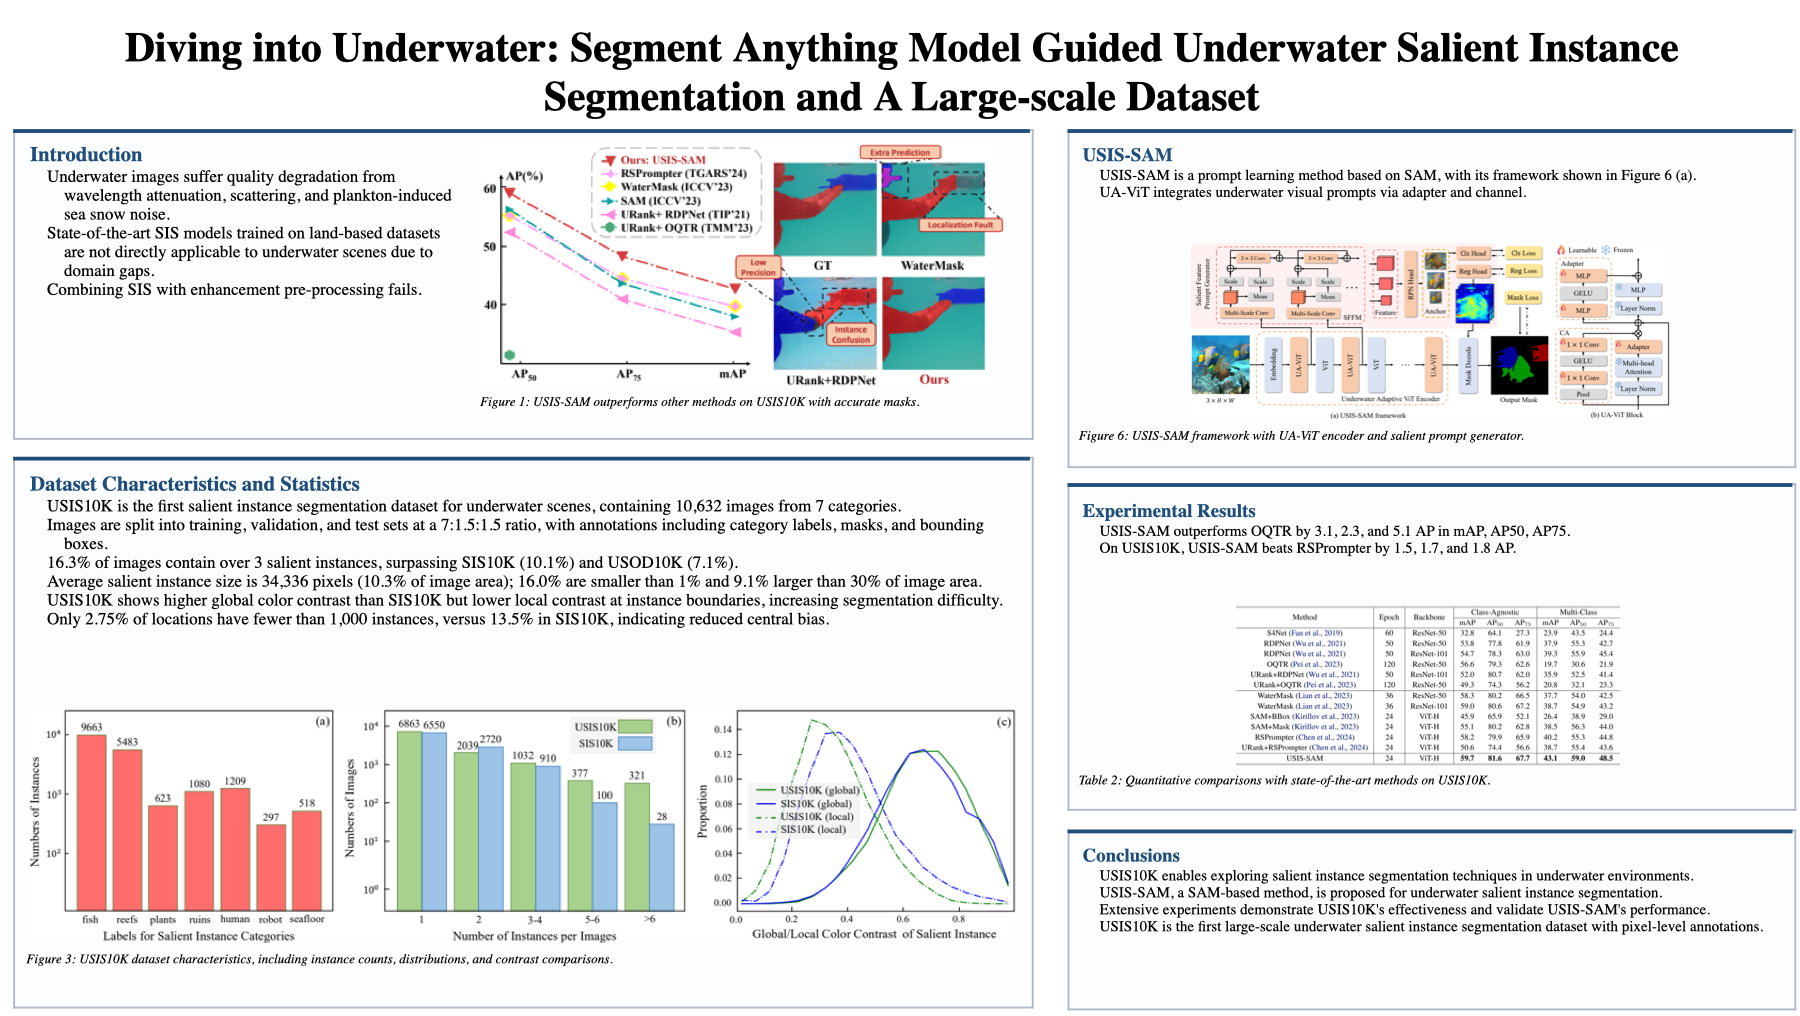
\includegraphics[width=0.88\textwidth]{figures/success_case_proposed.png}
}{
\fbox{
\parbox[c][7cm][c]{0.82\textwidth}{
\centering
Successful proposed-method poster example\
\textit{Diving into Underwater}
}
}
}
\caption{Representative successful poster generated by the proposed method.}
\label{fig:success_case}
\end{figure}

\vspace{1em}

Figure~\ref{fig:success_case} shows the final poster generated by the proposed method for this paper. This example is intended to illustrate that the system can produce a complete and readable single-page layout when the input structure is relatively stable, rather than to suggest that all papers can achieve the same generation quality.

\subsection{Comparative Case with the Fixed-Template Baseline}

To more directly examine the difference between dynamic layout generation and a fixed-template approach, this project further compares the two PPTX posters generated for \textit{GeoReasoner: Geo-localization with Reasoning in Street Views using a Large Vision-Language Model}. For this paper, the proposed method achieved an Overall Score of 79.576, whereas the template-based baseline achieved an Overall Score of 69.913, indicating a substantial performance gap between the two methods.

\vspace{1em}

The proposed method and the template-based baseline share the same main pipeline for content understanding and visual asset processing. Therefore, the difference in this case mainly comes from the subsequent layout strategy. A fixed template must place sections with different content volumes into predefined grid regions. When the sections vary substantially in text length, number of visual elements, and space requirements, such a fixed grid is more likely to produce local regions that are either overly crowded or insufficiently utilised.

\vspace{1em}

By contrast, the proposed method allocates space dynamically according to the textual content of each panel, the requirements of the associated visual assets, and the results of panel-level quality checks. It can also perform local content fitting when necessary. As a result, in this case, the proposed method produces a more balanced distribution of panel sizes and reduces the more obvious text crowding and unused space that appear in the fixed-template poster.

\begin{figure}[H]
\centering


\begin{minipage}[t]{0.48\textwidth}
    \centering
    \IfFileExists{figures/GeoReasoner_proposed.png}{
        \includegraphics[width=\textwidth]{figures/GeoReasoner_proposed.png}
    }{
        \fbox{
            \parbox[c][6cm][c]{0.9\textwidth}{
                \centering
                Proposed method\\
                GeoReasoner poster
            }
        }
    }

    \vspace{0.3em}
    \textbf{(a) Proposed method}
\end{minipage}
\hfill
\begin{minipage}[t]{0.48\textwidth}
    \centering
    \IfFileExists{figures/GeoReasoner_template.png}{
        \includegraphics[width=\textwidth]{figures/GeoReasoner_template.png}
    }{
        \fbox{
            \parbox[c][6cm][c]{0.9\textwidth}{
                \centering
                Template-based baseline\\
                GeoReasoner poster
            }
        }
    }

    \vspace{0.3em}
    \textbf{(b) Template-based baseline}
\end{minipage}

\caption{Comparison between the proposed method and the template-based baseline on the GeoReasoner paper.}
\label{fig:GeoReasoner_comparison}


\end{figure}

Figure~\ref{fig:GeoReasoner_comparison} provides a direct visual illustration of the difference between the two layout strategies. This case is consistent with the overall trend of the Rule Score on the selected set, namely that for papers with more uneven content structures, dynamic layout generation can better adapt to the actual space requirements of different panels than a fixed-template approach.

\vspace{1em}

It should be noted, however, that this example alone does not prove that dynamic layout generation is better than fixed templates for all papers. On the random set, the Rule Scores of the two PPTX-based methods are very similar, which suggests that fixed templates can also produce stable layouts for papers with more regular content structures. Therefore, this case is better interpreted as illustrating the advantage of dynamic layout generation on some complex samples, rather than as evidence for a universal conclusion.


\section{Summary of Results}

Across the two test sets, the three generation methods show clear differences across the evaluation dimensions, and no single method consistently performs best on all metrics. In terms of content evaluation, the Template-based baseline achieves the highest average Content Score, while the Proposed method performs at a similar level. Compared with the Direct LLM baseline, the Proposed method performs better on the detail questions, indicating that its generated posters preserve more specific information from the original papers, including methodological details, experimental settings, and reported results. At the same time, the differences among the three methods on the understanding questions are relatively small, suggesting that all three approaches are generally able to communicate the high-level research objectives and main conclusions of the papers.

\vspace{1em}

In terms of factual faithfulness, the Direct LLM baseline achieves the highest Faithfulness Score, while the Proposed method and the Template-based baseline obtain similar results. When considered together with the Content Score, this shows that higher factual faithfulness does not necessarily mean that more information from the original paper has been retained. The Direct LLM baseline tends to generate more concise and conservative content, which reduces the number of specific claims that may be unsupported by the source paper, but also increases the likelihood that paper-specific details are omitted. By contrast, the Proposed method retains more specific information, and therefore the Content and Faithfulness metrics need to be interpreted together.

\vspace{1em}

For visual quality and layout, the advantage of the Proposed method over the Template-based baseline is mainly observed on the selected set. For papers with more uneven content structures and visual requirements, dynamic space allocation, panel quality checking, and content fitting reduce more obvious text overflow and excessive whitespace. However, on the random set, the two PPTX-based methods produce very similar layout results, indicating that fixed templates can also provide stable performance for papers with relatively regular structures. The Direct LLM baseline achieves the highest average Overall Score and Visual Score, although its HTML output uses a different layout and rendering mechanism from the PPTX-based methods and should therefore be interpreted with this difference in mind.

\vspace{1em}

Overall, the experimental results indicate that the three methods reflect different design priorities. The main strengths of the Proposed method lie in preserving paper-specific information and adapting the layout to uneven content structures. The Template-based baseline provides stable results for more regular structures, while the Direct LLM baseline remains competitive in factual faithfulness and overall visual scoring. Paper-to-poster generation therefore involves practical trade-offs between content coverage, factual accuracy, and visual presentation, and a single aggregate score is insufficient to fully characterise the strengths and weaknesses of different generation approaches.

%%%%%%%%%%%%%%%%%%%%%%%%%%%%%%%%%%%%%%%%%%%%%%%%%%%%%%%%%%%%%%%%%%%%%%%%%%%%%

\chapter{Discussion and Limitations}

\section{Main Findings and Discussion}

The experimental results first suggest that structured content processing has practical value for single-page academic poster generation. When a full research paper is compressed into a poster, the information most likely to be lost is often not the high-level research objective, but finer-grained details such as method components, datasets, experimental settings, and specific results. The Proposed method performs better than the Direct LLM baseline on the detail questions, suggesting that explicitly conducting section selection, key-fact preservation, and poster-oriented summarisation before final poster generation can reduce the loss of paper-specific details during compression. Paper-to-poster generation should therefore not be understood simply as ordinary text summarisation, but rather as a structured generation task that requires active selection and reorganisation of research information.

\vspace{1em}

The experiments also show that information coverage and factual faithfulness are related but distinct objectives. More concise and conservative posters usually contain fewer specific claims, which reduces the opportunities for factual deviation. In contrast, retaining more methodological details and experimental results can increase the amount of useful information, but also requires additional compression and rewriting, creating more opportunities for local changes in expression. Optimising Faithfulness alone therefore does not guarantee that a poster contains enough useful information, while increasing information density without sufficient control may affect factual reliability and readability. For academic poster generation, Content Score and Faithfulness Score are better treated as complementary measures rather than interchangeable indicators of quality.

\vspace{1em}

The layout results further indicate that the main value of dynamic layout generation is not that it universally outperforms fixed templates, but that it improves adaptability to different content structures. When the textual and visual requirements of different sections are relatively balanced, a fixed template can already provide stable spatial organisation, leaving limited room for dynamic layout to improve the result. In contrast, when the spatial requirements of different panels vary substantially, predefined grids are more likely to produce local crowding or inefficient use of space, whereas content-aware allocation can respond to the actual requirements of each panel. The dynamic layout strategy developed in this project is therefore better understood as a mechanism for improving adaptability rather than as a universal replacement for fixed templates.

\vspace{1em}

The modular architecture also provides stronger inspectability. Compared with one-step generation, intermediate representations make it possible to associate content omissions, visual asset problems, and layout failures with specific processing stages such as PDF parsing, section selection, asset matching, or layout generation. This increases implementation complexity, but it also makes individual modules easier to inspect, replace, and improve. For a task that combines document understanding, text generation, visual asset organisation, and two-dimensional layout, this traceability is one of the practical advantages of a modular approach.

\section{System Limitations}

The main upstream limitation of the current system remains PDF parsing. The system relies on Docling to convert the original paper into a structured representation, which then forms the basis for subsequent section selection, summarisation, visual asset processing, and layout generation. For digital papers with normal text layers and common academic layouts, this process can usually provide relatively complete information. However, complex multi-column structures, irregular section headings, unusual captions, and complex tables may still lead to parsing errors. Because downstream modules directly use these structured results, upstream recognition errors may propagate into content selection and figure-text matching. The modular architecture helps identify where such problems occur, but it cannot automatically recover all incorrectly parsed information.

\vspace{1em}

A second limitation arises from the unavoidable information compression between a full research paper and a single-page poster. The methodological details, experimental settings, numerical results, and supplementary explanations contained in a complete paper greatly exceed the amount of information that can be displayed on one page. The system must therefore decide which information to retain and which to omit. The current implementation uses section selection, key facts, and poster-oriented summarisation to preserve important information and applies content fitting during layout generation to adjust information density. However, these mechanisms cannot eliminate the fundamental trade-off between information coverage and page readability. Preserving more detail can make the page overcrowded, while further compression increases the risk that important facts are omitted.

\vspace{1em}

A third limitation is the heuristic nature of the current layout strategy. The system estimates spatial requirements from text length, visual asset demand, panel role, and aspect ratio, and uses panel quality checks and limited refinement to reduce obvious overflow and excessive whitespace. The experiments show that this approach can improve layout adaptability for some complex papers, but these estimates cannot fully predict the final spatial requirements after rendering in PowerPoint. For papers with very high information density, many visual assets, or unusually shaped figures, the initial spatial estimates may still differ from the final rendered result. The current approach should therefore be regarded as an interpretable and controllable layout heuristic rather than an optimisation method that guarantees a globally optimal layout.

\section{Evaluation Limitations}

This project evaluates 40 papers using separate selected and random test sets. This scale is sufficient to observe the main trends of the current prototype and its baselines, but it is not large enough to represent all research fields and paper structures. Papers from different disciplines may vary substantially in formula density, visual asset types, section organisation, and presentation conventions. The current results therefore support the feasibility of the system within the evaluated scope, rather than demonstrating that the same level of performance would be achieved across all academic domains.

\vspace{1em}

PaperQuiz provides a content evaluation approach that is closer to how readers recover information from a poster than simple text-similarity metrics. However, its coverage is still limited by the available question set. If an important piece of information from the paper is not covered by any question, omitting it from the poster does not directly reduce the Content Score. In addition, detail and understanding questions may not have identical levels of difficulty. Their averaged accuracy is therefore more appropriately interpreted as a practical measure of content communication rather than an absolute measure of how completely the poster represents the original paper.

\vspace{1em}

The Faithfulness Score also has a clear evaluation boundary. It checks whether factual claims that appear in the poster are supported by the original paper, but it does not directly penalise omitted information. A poster containing only a small number of conservative claims may therefore obtain a high Faithfulness Score while still providing insufficient information. This project reports Content and Faithfulness separately in order to distinguish between whether the generated statements are correct and whether the poster contains enough useful information.

\vspace{1em}

The Visual Score is also limited by both the VLM evaluator and the rule-based checks. VLM-as-Judge can assess the overall layout, information hierarchy, and visual appeal of a complete poster, but its judgements remain partly subjective. Rule-based evaluation can consistently identify concrete problems such as overflow, out-of-bounds elements, excessive whitespace, and overly small visual assets, but it cannot fully assess typography, visual focus, or discipline-specific design conventions. The current Visual Score should therefore be understood as a combined approximation based on multiple visual signals rather than a complete substitute for human design evaluation.

\vspace{1em}

In addition, the Direct LLM baseline outputs HTML, whereas the Proposed method and the Template-based baseline output PPTX. Although all three results are rendered into images before evaluation, HTML/CSS and PowerPoint use different text-flow and layout mechanisms. The methods are therefore not compared under completely identical underlying rendering conditions. The visual metrics are suitable for comparing final visible outputs, but they should not be interpreted as a strictly controlled comparison of layout algorithms under the same rendering technology.

\vspace{1em}

Finally, the Overall Score uses an equal average of Content, Faithfulness, and Visual Scores to provide a convenient aggregate comparison. This does not imply that the three dimensions have exactly the same importance in all practical scenarios. Formal academic dissemination may place greater emphasis on factual reliability, while conference presentation may place more emphasis on rapid understanding and visual readability. The Overall Score should therefore be interpreted together with the individual sub-scores rather than used as the sole criterion for judging system quality.

\section{Practical Significance and Usage Boundaries}

From the perspective of a real poster-creation workflow, the system is better suited to functioning as an academic poster drafting tool than as a fully autonomous publishing system. Creating a poster from a complete research paper requires content selection, summarisation, figure selection, text--visual organisation, and layout planning, and a substantial part of this process is repetitive. The current system can automate these initial stages and generate an editable PPTX draft containing the main textual content, visual assets, and page structure. Users can then modify the content emphasis, remove unnecessary information, replace visual materials, and adjust fonts, colours, and panel positions according to the requirements of a particular conference or research group.

\vspace{1em}

This workflow also defines the responsibility boundary of the system. Automatically generated posters should not be used for formal academic dissemination without author verification. Summary generation, caption rewriting, and local content fitting may alter the wording of the source material, and figure-text matching may omit or incorrectly infer some relationships. Even though the overall Faithfulness Scores in the experiments are relatively high, key numerical results, major conclusions, method descriptions, and visual asset associations should still be checked by the author before publication or presentation.

\vspace{1em}

The system is therefore best understood as a human-in-the-loop poster generation tool. Automation reduces the workload involved in moving from a complete paper to an initial poster draft, while the author retains responsibility for final content judgement and visual presentation. This positioning is also consistent with the PPTX output format: the system provides an editable starting point rather than attempting to replace the researcher in the final design process.

\section{Future Work}

One important direction for future work is to analyse system performance more systematically across different paper types and levels of structural complexity. The current experiments show that the advantage of the Proposed method over the fixed-template baseline is more apparent on the selected set and smaller on the random set. Future evaluation could group papers according to characteristics such as paper type, number of sections, text density, number of visual assets, and variation in panel space requirements. This would help identify more precisely which types of papers benefit most from dynamic layout generation.

\vspace{1em}

A second direction is to separate the effects of layout strategy, generation process, and output format more carefully. The current Direct LLM baseline uses HTML, whereas the other two methods use PPTX, so output format and generation architecture change at the same time. Future experiments could apply different layout strategies to the same structured assets or render the same content in both HTML and PPTX. This would make it possible to measure the contribution of dynamic layout generation more directly.

\vspace{1em}

The layout method itself also leaves room for further improvement. The current recursive binary-tree approach has the advantages of being structurally clear, interpretable, and easy to constrain, but its spatial allocation still depends on heuristic weights and loss functions. Future work could explore constrained optimisation or learning-based layout generation while preserving explicit controls such as minimum panel size, reading order, and content capacity. This may improve space utilisation and layout stability without sacrificing the controllability of the current system.

\vspace{1em}

Another useful direction is to provide greater user control. Different authors may wish to emphasise different aspects of the same paper. Future versions of the system could allow users to lock required sections or visual assets, adjust panel importance, specify a target poster size, or select different levels of information density. This would retain the benefits of automation while making the generated result better aligned with the author's intended research message.

\vspace{1em}

Finally, the practical value of the system should be evaluated through a real user study. The current automatic metrics primarily evaluate the generated poster itself and do not directly measure whether an editable poster draft reduces the time and effort required to create a final academic poster. Future work could compare a workflow in which researchers create posters from a blank page with one in which they refine an automatically generated PPTX draft. Completion time, number of manual modifications, proportion of automatically generated content retained, and subjective satisfaction could then be measured. Such an evaluation would provide a more direct assessment of the system's intended role as a tool for generating useful first drafts rather than fully automatic final posters.

%%%%%%%%%%%%%%%%%%%%%%%%%%%%%%%%%%%%%%%%%%%%%%%%%%%%%%%%%%%%%%%%%%%%%%%%%%%%%

\chapter{Conclusion}

This project designed and implemented a complete prototype system for converting research paper PDFs into editable PPTX academic posters. Paper parsing, section selection, content compression, visual asset organisation, figure-text matching, layout generation, and local content adaptation are organised into explicit processing stages and connected through unified intermediate representations. Compared with reducing the entire paper-to-poster task to a single model call, this modular structure allows content understanding, visual asset processing, and two-dimensional layout generation to be handled separately, while preserving key intermediate states that make the final output easier to inspect and adjust.

\vspace{1em}

The experimental results show that paper-to-poster generation cannot be judged effectively using a single metric. Clear trade-offs exist between content coverage, factual faithfulness, and visual quality. The Proposed method does not achieve the highest score on every automatic metric, but it preserves more paper-specific details than the Direct LLM baseline and shows stronger layout adaptability than the fixed-template baseline for papers with more uneven content structures and spatial requirements. The Direct LLM baseline remains competitive in Faithfulness Score and overall Visual Score, while fixed templates can still produce stable results for papers with more regular structures. These differences reflect different design priorities rather than a simple ranking of overall superiority.

\vspace{1em}

Overall, the project demonstrates the feasibility of a complete workflow for automatically converting academic papers into editable poster drafts. The value of the system lies not in replacing researchers in the final design process, but in automating the main content organisation, visual asset arrangement, and initial layout planning required to move from a complete paper to a usable poster draft, while preserving the possibility of further manual refinement. For academic poster generation, which requires factual accuracy, information compression, visual organisation, and final author control, a modular and inspectable generation process with editable output provides a practical implementation approach.




\cleardoublepage
\addcontentsline{toc}{chapter}{References}
\renewcommand{\bibname}{References}
\bibliographystyle{unsrt}
\bibliography{references}



\end{document}
